\documentclass[tikz,dvipdfmx]{standalone}
\usepackage{graphicx}

\usetikzlibrary{
  arrows.meta,
  positioning
}

\begin{document}
\begin{tikzpicture}
  \def\y{3}

  \node (A) at (-1.2*\y,0) {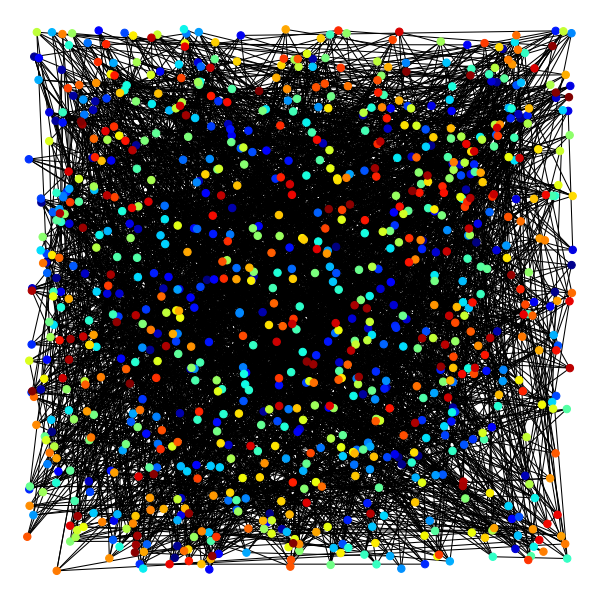
\includegraphics[width=3cm]{../individual/vis/fig1_init_random.png}};
  \node[above=0.1cm of A, scale=1.2] {\large{\textsf{random}}};

  \node (B) at (-1.8*\y,-5) {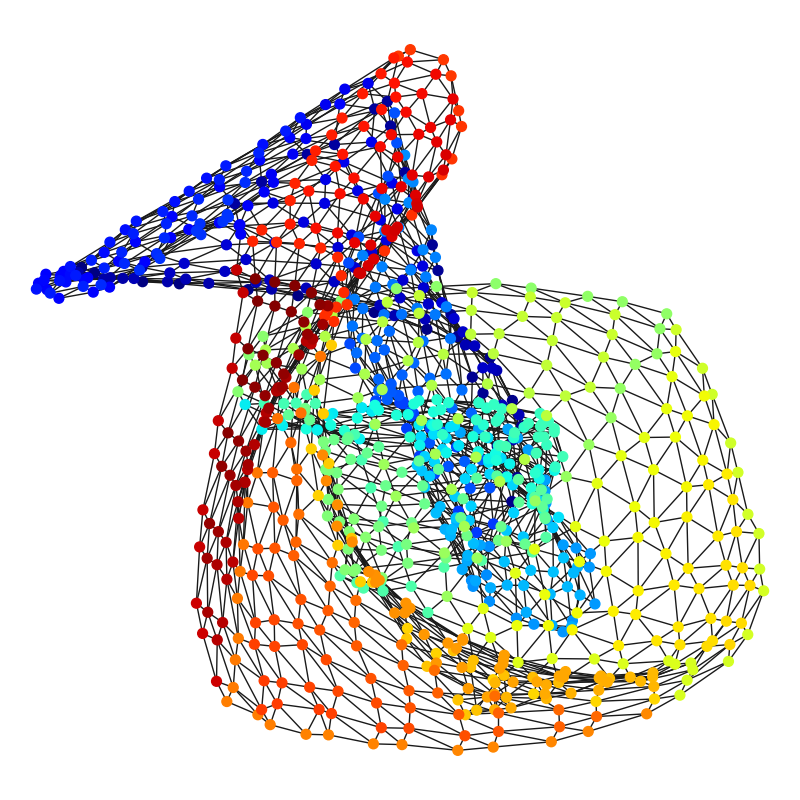
\includegraphics[width=3cm]{../individual/vis/jagmesh1_FR.png}};

  \node (C) at (-0.6*\y,-5) {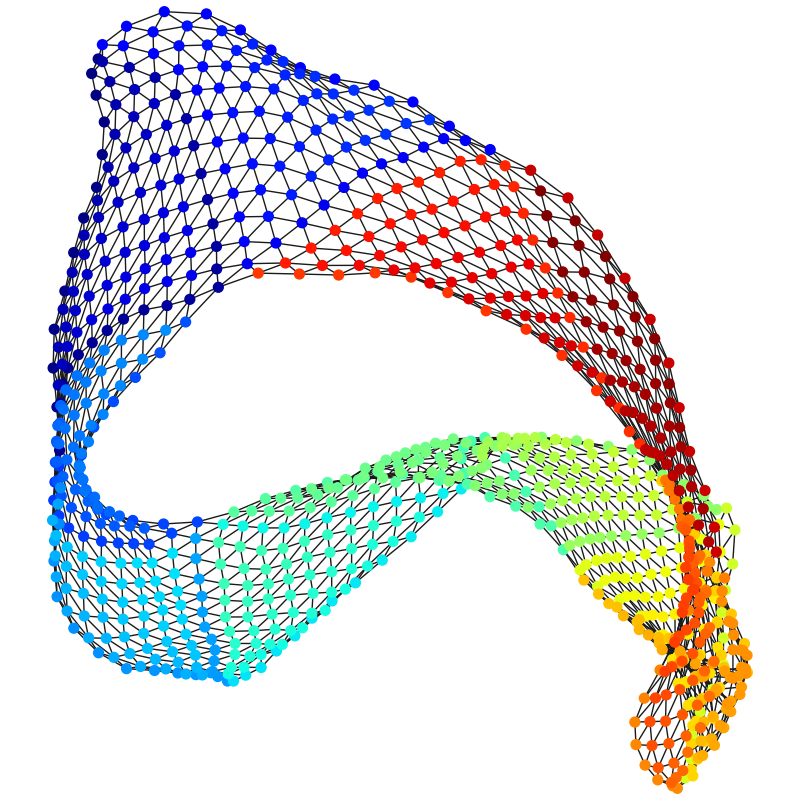
\includegraphics[width=3cm]{../individual/vis/jagmesh1_L-BFGS.png}};

  \node (D) at (+1.2*\y, 0) {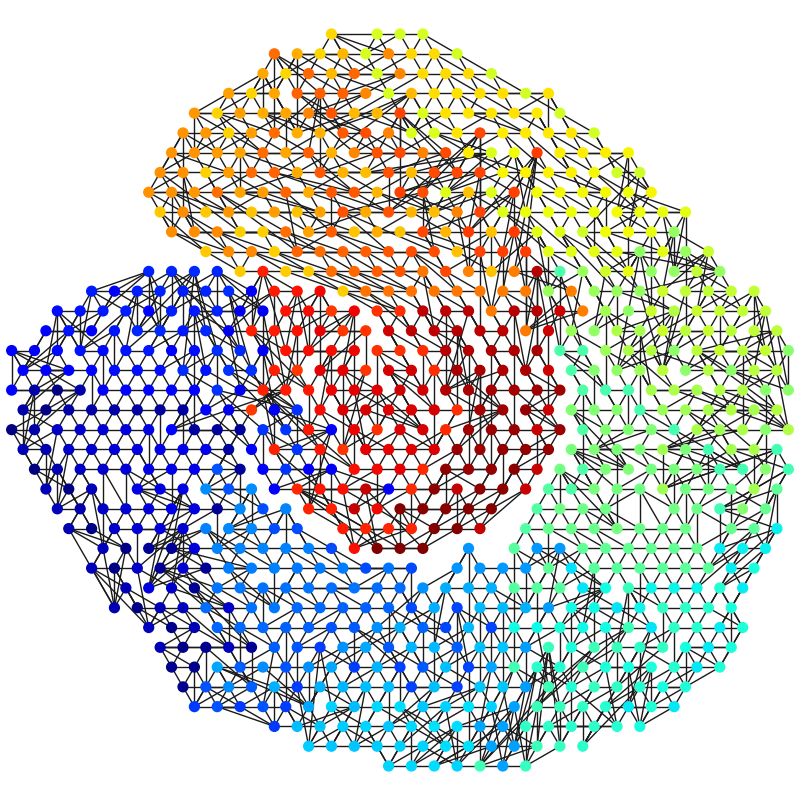
\includegraphics[width=3cm]{../individual/vis/fig1_init_CN.png}};
  \node[above=-0.1cm of D, scale=1.2] {\large{\textsf{initial placement}}};

  \node (E) at (+0.6*\y,-5) {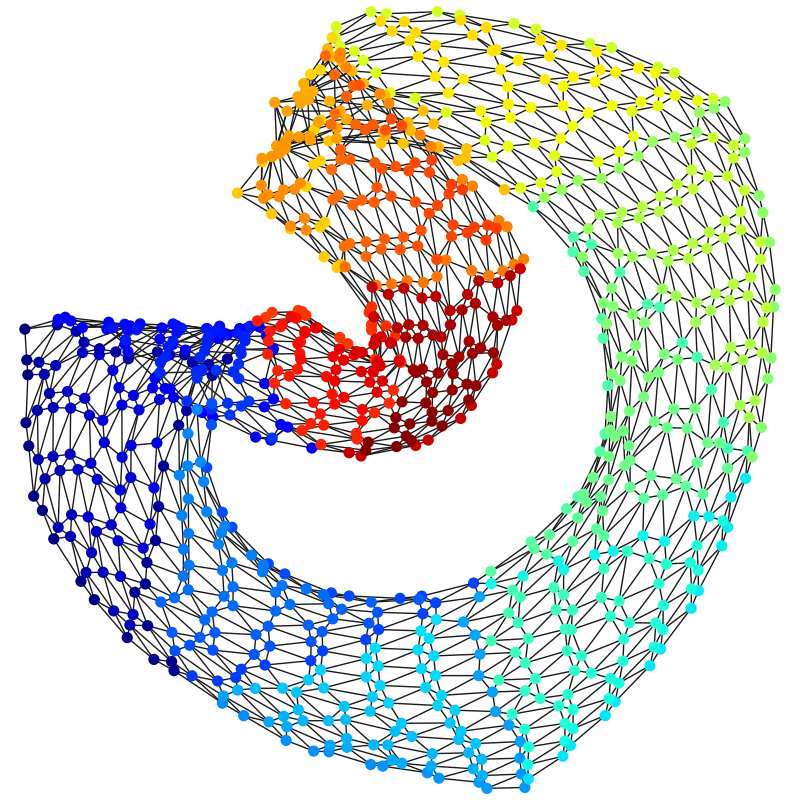
\includegraphics[width=3cm]{../individual/vis/jagmesh1_CN-FR.png}};

  \node (F) at (+1.8*\y,-5) {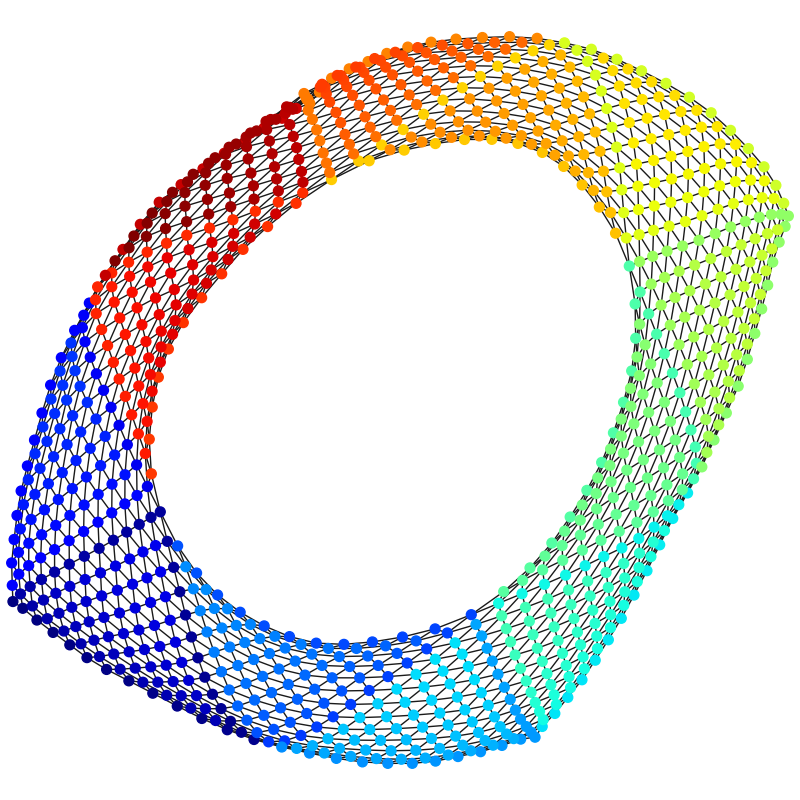
\includegraphics[width=3cm]{../individual/vis/jagmesh1_CN-L-BFGS.png}};

  % Draw arrows with labels
  \draw[-{Stealth[length=2mm,width=3mm]},line width=0.07cm] (A) -- (B) node[midway, left=0.4cm,scale=1.2] {\Large{\textsf{FR}}};
  \draw[-{Stealth[length=2mm,width=3mm]},line width=0.07cm] (A) -- (C) node[midway, right=0.4cm,scale=1.2] {\Large{\textsf{L-BFGS}}};
  \draw[-{Stealth[length=3mm,width=4mm]},line width=0.1cm, red] (A) -- (D) node[midway, below, red,scale=1.2] {\LARGE{\textbf{\textsf{proposed}}}};
  \draw[-{Stealth[length=2mm,width=3mm]},line width=0.07cm] (D) -- (E) node[midway, left=0.4cm,scale=1.2] {\Large{\textsf{FR}}};
  \draw[-{Stealth[length=2mm,width=3mm]},line width=0.07cm] (D) -- (F) node[midway, right=0.4cm,scale=1.2] {\Large{\textsf{L-BFGS}}};
\end{tikzpicture}
\end{document}
